\documentclass{beamer}
\usepackage[utf8]{inputenc}

\usetheme{Madrid}
\usecolortheme{default}
\usepackage{amsmath,amssymb,amsfonts,amsthm}
\usepackage{mathtools}
\usepackage{txfonts}
\usepackage{tkz-euclide}
\usepackage{listings}
\usepackage{adjustbox}
\usepackage{array}
\usepackage{gensymb}
\usepackage{tabularx}
\usepackage{gvv}
\usepackage{lmodern}
\usepackage{circuitikz}
\usepackage{tikz}
\lstset{literate={·}{{$\cdot$}}1 {λ}{{$\lambda$}}1 {→}{{$\to$}}1}
\usepackage{graphicx}

\setbeamertemplate{page number in head/foot}[totalframenumber]

\usepackage{tcolorbox}
\tcbuselibrary{minted,breakable,xparse,skins}



\definecolor{bg}{gray}{0.95}
\DeclareTCBListing{mintedbox}{O{}m!O{}}{%
  breakable=true,
  listing engine=minted,
  listing only,
  minted language=#2,
  minted style=default,
  minted options={%
    linenos,
    gobble=0,
    breaklines=true,
    breakafter=,,
    fontsize=\small,
    numbersep=8pt,
    #1},
  boxsep=0pt,
  left skip=0pt,
  right skip=0pt,
  left=25pt,
  right=0pt,
  top=3pt,
  bottom=3pt,
  arc=5pt,
  leftrule=0pt,
  rightrule=0pt,
  bottomrule=2pt,
  toprule=2pt,
  colback=bg,
  colframe=orange!70,
  enhanced,
  overlay={%
    \begin{tcbclipinterior}
    \fill[orange!20!white] (frame.south west) rectangle ([xshift=20pt]frame.north west);
    \end{tcbclipinterior}},
  #3,
}
\lstset{
    language=C,
    basicstyle=\ttfamily\small,
    keywordstyle=\color{blue},
    stringstyle=\color{orange},
    commentstyle=\color{green!60!black},
    numbers=left,
    numberstyle=\tiny\color{gray},
    breaklines=true,
    showstringspaces=false,
}
%------------------------------------------------------------
%This block of code defines the information to appear in the
%Title page
\title %optional
{4.13.31}
\date{September 4,2025}
%\subtitle{A short story}

\author % (optional)
{Harsha-EE25BTECH11026}



\begin{document}


\frame{\titlepage}


\begin{frame}{Question}
Line L has intercepts a and b on the coordinate axes. When the axes are rotated
through a given angle, keeping the origin fixed, line L has intercepts p and q. Then

\begin{enumerate}
    \item $a^2+b^2=p^2+q^2$
    \item $\frac{1}{a^2}+\frac{1}{b^2}=\frac{1}{p^2}+\frac{1}{q^2}$
    \item $a^2+p^2=b^2+q^2$
    \item $\frac{1}{a^2}+\frac{1}{p^2}=\frac{1}{b^2}+\frac{1}{q^2}$
\end{enumerate}

\end{frame}

\begin{frame}{Theoretical Solution}
According to the question,\\
\begin{align}
    \text{The equation of line\,:\,}\myvec{\frac{1}{a}&&\frac{1}{b}}\vec{x}=1
\end{align} 
Let the row coefficient vector of the original line be $\vec{m}$ and for the rotated line be $\vec{m'}$.

\begin{align}
     \vec{m'}=\vec{P}\vec{m}       
\end{align}
where $\vec{P}$ is the rotation matrix
\end{frame}

\begin{frame}{Equation}
\begin{align}
    \|\vec{m'}\|^2=\vec{m'}^{\top}\vec{m'}=\brak{\vec{m}^{\top}\vec{P}^{\top}}\brak{\vec{P}\vec{m}}=\vec{m}^{\top}\brak{\vec{P}^{\top}\vec{P}}\vec{m}
\end{align}
Since $\vec{P}$ is an orthogonal matrix,
\begin{align}
    \therefore \vec{m}^{\top}\brak{\vec{P}^{\top}\vec{P}}\vec{m}=\vec{m}^{\top}\vec{m}=\|m\|^2
\end{align}
\begin{align}
    \implies \|\vec{m'}\|^2=\|\vec{m}\|^2
\end{align}
As $\vec{m'}$ is given by $\myvec{\frac{1}{p}&&\frac{1}{q}}^{\top}$,
\begin{align}
    \therefore \frac{1}{p^2}+\frac{1}{q^2}=\frac{1}{a^2}+\frac{1}{b^2}
\end{align}

\end{frame}


\begin{frame}[fragile]
    \frametitle{C Code -Finding Equation of the plane}

    \begin{lstlisting}
#include <stdio.h>
#include <math.h>

void line_intercepts_after_rotation(double a, double b, double theta, double *p, double *q) {
    // vector [1/a, 1/b]
    double m[2] = {1.0/a, 1.0/b};
    // Rotation matrix
    double P[2][2] = {
        {cos(theta), -sin(theta)},
        {sin(theta),  cos(theta)}
    };
    double m_new[2];
    m_new[0] = m[0]*P[0][0] + m[1]*P[1][0];
    m_new[1] = m[0]*P[0][1] + m[1]*P[1][1];
    *p = 1.0 / m_new[0];
    *q = 1.0 / m_new[1];
}


    \end{lstlisting}
\end{frame}

\begin{frame}[fragile]
    \frametitle{C Code -Finding Equation of the plane}

    \begin{lstlisting}
// Function to check options (returns index of true option)
int check_options(double a, double b, double p, double q, double eps) {
    double optA = fabs((a*a + b*b) - (p*p + q*q)) < eps;
    double optB = fabs((1.0/(a*a) + 1.0/(b*b)) - (1.0/(p*p) + 1.0/(q*q))) < eps;
    double optC = fabs((a*a + p*p) - (b*b + q*q)) < eps;
    double optD = fabs((1.0/(a*a) + 1.0/(p*p)) - (1.0/(b*b) + 1.0/(q*q))) < eps;

    if(optA) return 1;
    if(optB) return 2;
    if(optC) return 3;
    if(optD) return 4;
    return 0; // none true
}

    \end{lstlisting}
\end{frame}

\begin{frame}[fragile]
    \frametitle{Python+C code}

    \begin{lstlisting}[language=Python]
import ctypes
import numpy as np
import matplotlib.pyplot as plt
import matplotlib as mp
mp.use("TkAgg")

# Load shared library
lib = ctypes.CDLL("./libline_rotation.so")

# Function signatures
lib.line_intercepts_after_rotation.argtypes = [
    ctypes.c_double, ctypes.c_double, ctypes.c_double,
    ctypes.POINTER(ctypes.c_double), ctypes.POINTER(ctypes.c_double)
]
lib.line_intercepts_after_rotation.restype = None


    \end{lstlisting}
\end{frame}

\begin{frame}[fragile]
    \frametitle{Python+C code}

    \begin{lstlisting}[language=Python]
lib.check_options.argtypes = [
    ctypes.c_double, ctypes.c_double,
    ctypes.c_double, ctypes.c_double, ctypes.c_double
]
lib.check_options.restype = ctypes.c_int
# Parameters
a, b = 3.0, 4.0
theta = np.pi / 3
# Call C function to compute new intercepts
p, q = ctypes.c_double(), ctypes.c_double()
lib.line_intercepts_after_rotation(a, b, theta, ctypes.byref(p), ctypes.byref(q))
p, q = p.value, q.value
# Check which option is true
opt = lib.check_options(a, b, p, q, 1e-8)
print(f"Correct Option: {opt}")

    \end{lstlisting}
\end{frame}

\begin{frame}[fragile]
    \frametitle{Python+C code}

    \begin{lstlisting}[language=Python]
# ========== PLOT ONLY IF OPTION B IS TRUE ==========
if opt == 2:
    # Original line
    x_vals = np.linspace(-1, max(a, 6), 400)
    y_vals = b * (1 - x_vals / a)
    # Original intercepts
    A = (a, 0)
    B = (0, b)
    # Rotated axes directions
    e1_new = np.array([np.cos(theta), np.sin(theta)])
    e2_new = np.array([-np.sin(theta), np.cos(theta)])
    # Transform new intercepts (rotated -> original coords)
    P = np.array([
        [np.cos(theta), -np.sin(theta)],
        [np.sin(theta),  np.cos(theta)]
    ])
    Pp = P @ np.array([p, 0])
    Pq = P @ np.array([0, q])

    \end{lstlisting}
\end{frame}

\begin{frame}[fragile]
    \frametitle{Python+C code}

    \begin{lstlisting}[language=Python]
   # Plot
    plt.figure(figsize=(7,7))
    plt.axhline(0, color='gray', lw=1)
    plt.axvline(0, color='gray', lw=1)
    plt.plot(x_vals, y_vals, 'b', label="Original line")
    plt.scatter(*A, color='blue')
    plt.text(A[0], A[1]-0.3, f"A({a:.3f},0)", ha='center', fontsize=10, color="blue")
    plt.scatter(*B, color='blue')
    plt.text(B[0]-0.3, B[1], f"B(0,{b:.3f})", va='center', fontsize=10, color="blue")
    t = np.linspace(-6, 6, 200)
    plt.plot(t*e1_new[0], t*e1_new[1], 'r--', label="Rotated X'-axis")
    plt.plot(t*e2_new[0], t*e2_new[1], 'r--', label="Rotated Y'-axis")

 

    \end{lstlisting}
    
\end{frame}

\begin{frame}[fragile]
    \frametitle{Python+C code}

    \begin{lstlisting}[language=Python]
  # New intercepts (P, Q)
    plt.scatter(*Pp, color='green')
    plt.text(Pp[0], Pp[1]-0.2, f"P({p:.3f},0)", color='green', ha='center', fontsize=10)

    plt.scatter(*Pq, color='green')
    plt.text(Pq[0]-0.2, Pq[1], f"Q(0,{q:.3f})", color='green', va='center', fontsize=10)

    plt.axis("equal")
    plt.legend(loc="upper right")
    plt.title("Graph for the True Relation:\n1/a² + 1/b² = 1/p² + 1/q²")
    plt.savefig("/home/user/Matrix/Matgeo_assignments/4.13.31/figs/Figure_1")
    plt.show()



    \end{lstlisting}
    
\end{frame}



\begin{frame}[fragile]
    \frametitle{Python code}

    \begin{lstlisting}[language=Python]
import numpy as np
import matplotlib.pyplot as plt
import matplotlib as mp
mp.use("TkAgg")

def line_intercepts_after_rotation(a, b, theta):
    m = np.array([1/a, 1/b])
    P = np.array([
        [np.cos(theta), -np.sin(theta)],
        [np.sin(theta),  np.cos(theta)]
    ])
    m_new = m @ P
    return 1/m_new[0], 1/m_new[1]   # p, q

    \end{lstlisting}
    
\end{frame}

\begin{frame}[fragile]
    \frametitle{Python code}

    \begin{lstlisting}[language=Python]
# Parameters
a, b = 3, 4
theta = np.pi/3
# New intercepts
p, q = line_intercepts_after_rotation(a, b, theta)
# ========== BOOLEAN CHECK SECTION ==========
eps = 1e-8

optA = abs((a**2 + b**2) - (p**2 + q**2)) < eps
optB = abs((1/a**2 + 1/b**2) - (1/p**2 + 1/q**2)) < eps
optC = abs((a**2 + p**2) - (b**2 + q**2)) < eps
optD = abs((1/a**2 + 1/p**2) - (1/b**2 + 1/q**2)) < eps

print(f"Option A : {optA}")
print(f"Option B : {optB}")
print(f"Option C : {optC}")
print(f"Option D : {optD}")
    \end{lstlisting}
    
\end{frame}

\begin{frame}[fragile]
    \frametitle{Python code}

    \begin{lstlisting}[language=Python]
if optB:   # Only plot when option B is satisfied
    # Original line
    x_vals = np.linspace(-1, max(a, 6), 400)
    y_vals = b*(1 - x_vals/a)
    # Original intercepts
    A = (a,0)
    B = (0,b)
    # Rotated axes directions
    e1_new = np.array([np.cos(theta), np.sin(theta)])
    e2_new = np.array([-np.sin(theta), np.cos(theta)])
    # Transform new intercepts (in rotated coords) back to old coords
    P = np.array([[np.cos(theta), -np.sin(theta)],
                  [np.sin(theta),  np.cos(theta)]])
    Pp = P @ np.array([p,0])   # (p,0) in rotated coords
    Pq = P @ np.array([0,q])   # (0,q) in rotated coords
    \end{lstlisting}
    
\end{frame}

\begin{frame}[fragile]
    \frametitle{Python code}

    \begin{lstlisting}[language=Python]
    # Plot
    plt.figure(figsize=(7,7))
    plt.axhline(0, color='gray', lw=1)
    plt.axvline(0, color='gray', lw=1)
    # Original line
    plt.plot(x_vals, y_vals, 'b', label="Original line")
    # Original intercepts
    plt.scatter(*A, color='blue')
    plt.scatter(*B, color='blue')
    plt.text(A[0], A[1]-0.3, f"A({a},0)", ha='center')
    plt.text(B[0]-0.3, B[1], f"B(0,{b})", va='center')
    # Draw rotated axes as extended lines
    t = np.linspace(-6, 6, 200)
    plt.plot(t*e1_new[0], t*e1_new[1], 'r--', label="Rotated X'-axis")
    plt.plot(t*e2_new[0], t*e2_new[1], 'r--', label="Rotated Y'-axis")

    \end{lstlisting}
    
\end{frame}

\begin{frame}[fragile]
    \frametitle{Python code}

    \begin{lstlisting}[language=Python]
  # New intercepts on rotated axes
    plt.scatter(*Pp, color='green')
    plt.scatter(*Pq, color='green')
    plt.text(Pp[0], Pp[1]-0.2, f"P({p:.2f},0)", color='green', ha='center')
    plt.text(Pq[0]-0.2, Pq[1], f"Q(0,{q:.2f})", color='green', va='center')

    plt.axis("equal")
    plt.legend()
    plt.title("Graph for the True Relation: 1/a² + 1/b² = 1/p² + 1/q²")
    plt.savefig("/home/user/Matrix/Matgeo_assignments/4.13.31/figs/Figure_1")
    plt.show()
    \end{lstlisting}
    
\end{frame}

\begin{frame}{Plot}
    \begin{figure}[H]
    \centering
    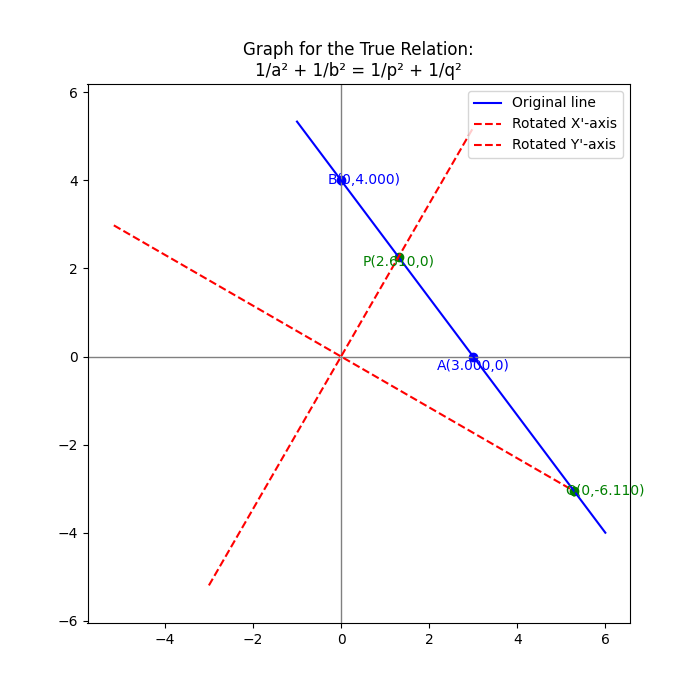
\includegraphics[width=0.6\columnwidth]{figs/Figure_1.png}
    \label{fig:1}
\end{figure}
\end{frame}

\end{document}